\setchapterpreamble[u]{\margintoc}
\chapter{Protocolli vari}
\labch{chapter12}


 \section{Bit commitment}

Supponiamo di trovarci nel caso un cui un agente conosca l'andamento della borsa nel futuro e inserisca questa informazione in una busta chiusa, che verrà aperta tra un anno. Vogliamo tentare di costruire il concetto di busta chiusa con i bit. Supponiamo di lavorare con singoli bit in quanto, se siamo in grado di "imbustare" un bit, possiamo farlo anche con sequenze di bit (es: concateniamo buste chiuse nell'ordine corretto).

Chiunque abbia davanti a se un bit in busta chiusa deve poter indovinare quel bit con probabilità $\frac{1}{2}$. Definiamo ora i requisiti che il protocollo deve soddisfare.


\paragraph{Creazione della busta:} $A$ invia un messaggio $m$ a $B$ tale per cui:
\begin{itemize}
    \item $m$ deve contenere un bit $b$ fissato;
    \item $A$ non deve essere in grado di cambiare $b$;
    \item $B$ non deve essere in grado di indovinare $b$\sidenote{Se noi costruiamo un algoritmo dove: Alice sceglie il bit $b$, genera il messaggio $m$, lo invia a Bob e Bob applica un qualche algoritmo per produrre un nuovo bit, la probabilità che questo sia uguale a $b$ differisce da $\frac{1}{2}$ di una quantità più piccola di ogni polinomio}.
\end{itemize}
    
\paragraph{Apertura della busta: } $A$ invia un messaggio $m'$ a $B$ tale per cui:
\begin{itemize}
    \item $B$ riesce a ricavare il bit $b$ da $m$ e $m'$;
    \item $A$ non deve riuscire a creare due coppie $(m, m')$ $(m, m'')$ che portano $B$ ad ottenere due risultati diversi.
\end{itemize}

\subsection{Protocollo 1}

Vediamo ora una prima implementazione del protocollo.

\begin{enumerate}
    \item $B$ invia ad $A$ un numero $R$ random (\textbf{nonce}\sidenote{Usato per autenticare l'agente. Il nonce è un number once, ovvero un numero mai usato in precedenza. Il modo più semplice per generarlo è generare una sequenza di bit a caso: se questa è sufficientemente lunga, la probabilità che esistano due agenti che abbiano usato lo stesso numero è più piccola di ogni polinomio.});
    \item $A$ invia a $B$ $E_k(Rb)$, ovvero la codifica con chiave $k$ della sequenza $Rb$, dove $k$ è una chiave casuale e $E$ è un algoritmo di crittografia simmetrica;
    \item $B$ conosce ora il cyphertext, eccetto per un bit. Tuttavia DES e AES non sono vulnerabili al known plaintext attack. In realtà non abbiamo usa dimostrazione che effettivamente non siano vulnerabili, ma tutte le analisi fatte fino ad ora ci portano a dire che non è possibile ricavare la chiave anche se conosciamo il plaintext di un dato cyphertext. Di conseguenza $B$ non ha modo di ricavare $b$, tranne provare tutte le possibili chiavi (attacco a forza bruta);
    \item $A$ invia $k$ a $B$;
    \item $B$ decodifica il messaggio e verifica che il contenuto del messaggio eccetto l'ultimo bit sia identico a $R$. 
\end{enumerate}

\noindent In questa implementazione $A$ non può imbrogliare in quanto dovrebbe trovare due chiavi $k_0, k_1$ tali per cui:
\begin{align*}
    E_k_0(R, 0) = E_k_1(R, 1)
\end{align*}
\noindent cioè dovrebbe trovare due chiavi tali per cui una permetta di aprire la busto rivelando il bit $0$, mentre la seconda permetta di aprire la busta rivelando il bit $1$ (su AES non siamo in grado di farlo).
\\

\noindent Questa soluzione presenta però due problemi:
\begin{itemize}
    \item Abbiamo detto che "non conosciamo altro metodo per" ricavare la chiave senza provarle tutte e per generare due chiave tali per cui una rivela $0$ e l'altra $1$. Abbiamo sempre detto che non è buona cosa usare un protocollo solo perché non siamo in grado di attaccarlo, quindi sarebbe meglio trovare qualcosa di dimostrabilmente sicuro;
    \item $A$ per creare la busta chiusa necessita del supporto di $B$, che deve generare $R$\sidenote{senza $R$ il messaggio diventerebbe arbitrario - contiene solo il bit scelto da $A$ - e quindi creare buste con valori diversi sarebbe banale, in quanto metà delle chiavi decodificherebbero un cyphertext come $0$ e l'altra $1$}. Se $B$ non invia $R$, $A$ non può inviare il bit.
\end{itemize}

\subsection{Protocollo 2}
Sia $H$ una funzione hash one way. Allora il protocollo è implementato come segue:
\begin{itemize}
    \item $A$ invia a $B$ $H(R_1 \ R_2 \ b), R_1$. $R_10$ e $R_2$ sono sequenze di bit casuali;
    \item $A$ invia a $B$ $R_2, b$ per aprire la busta.
\end{itemize}

\noindent Con il primo messaggio conosce l'hash del messaggio più parte del suo contenuto. L'unico modo che ha ora per ricavare il messaggio è invertire la funzione $H$. Se non fosse presente $R_2$, a $B$ basterebbe calcolare $H(R_1 \ 0)$ e $H(R_1 \ 1)$ per scoprire il valore del bit $b$.

Quando riceve il secondo messaggio, $B$ può calcolarne l'hash e verificare che $A$ non stia mentendo.

$A$ non è in grado di creare una busta che riveli due bit in quanto dovrebbe creare una situazione in cui:
\begin{align*}
    H(R_1 \ R_2 \ 0) = H(R_1 \ R_2' \ 1)
\end{align*}

\noindent Questo equivale a trovare conflitti nella funzione $H$, cosa che non siamo in grado di fare. 
\\

\noindent Siamo riusciti a creare un protocollo dove non è necessario che $B$ partecipi alla creazione della busta. Sia in questo protocollo che nel precedente possiamo sostituire il bit con una sequenza di bit. Anche questo protocollo non è dimostrabilmente sicuro.

\subsection{Protocollo 3}
Vediamo ora un protocollo dimostrabilmente sicuri che però richiede la collaborazione di $B$. Sarà molto complesso (a livello di complessità) e richiederà al sua applicazione ad ogni bit che si vuole "imbustare". Vediamo come funziona:
\begin{itemize}
    \item $B$ invia ad $A$ $R$, dove $R=r_1 \ ... \ r_l$;
    \item $A$ genera un seme $s$ e una pseudostringa di bit $X = x_1 \ ... \ x_l$. Genera poi:
    \begin{align*}
        \forall i \ y_i = \begin{cases} 
            x_i & \mbox{se }r_i = 0 \\ 
            x_i \oplus b & \mbox{se }r_i = 1
        \end{cases} 
    \end{align*}
    Invia a $B$ $y_1 \ ... \ y_l$. La sequenza $Y$ è una sequenza di bit generati o in modo pseudocasuale o messi in XOR col bit $b$. Nel momento in cui una quantità casuale viene messa in XOR con qualcosa, il risultato è casuale. Quindi se gli $x_i$ sono veramente casuali, allora la sequenza degli $y_i$ è anch'essa casuale. Ciò significherebbe che non contiene alcuna informazione circa il bit $b$.

    La sequenza $X$ è pseudocasuale. Se $B$ fosse in grado di ricavare dalla sequenza $Y$ informazioni circa il bit $b$, allora l'algoritmo per ricavare $b$ sarebbe un distinguisher per il generatore di bit pseudocasuali. 
    
    Il messaggio che $A$ invia non rivela quindi il bit $b$;
    \item $A$ invia a $B$ il seme $s$. $B$ diventa in grado di costruire ora la sequenza $X$ e verificare che tutti gli $y_i$ siano stati costruiti correttamente. 
\end{itemize}

\noindent Se tutti gli $r_i$ dovessero valere $0$, allora in nessuno degli $y_i$ sarebbe presenta l'informazione riguardo il bit $b$. Ma la probabilità che questo avvenga è $\frac{1}{2^l}$, trascurabile. 
\\

\noindent $A$ non può creare due buste in dovrebbe trovare due semi $s_0$ e $s_1$, tali per cui il primo porta alla stringa $x_1 \ ... \ x_l$ e il secondo alla stringa $x_1' \ ... \ x_l'$ e :
\begin{align*}
    \forall i \ \text{se } r_i = 1 \text{ allora } x_i = \overline{x_i'}
\end{align*}

\noindent ovvero:
\begin{align*}
    0 \oplus x_i = 1 \oplus x_i'
\end{align*}

\noindent Questa cosa è dimostrabile, anche se non lo facciamo. 

\section{Schemi a barriera}

Supponiamo di conoscere un segreto (es: chiave che sblocca gli armamenti nucleari) $s$, che è una sequenza di bit. Lo distribuiamo a $n$ agenti creando delle parti (\textbf{share}) $s_1 \ ... \ s_n$. Nessuno degli agenti possiede il segreto completo, ma solo un pezzo, in modo che mettendo assieme tutte le parti si ricava $S$. Mettendo assieme meno di $n$ parti, non si conosce niente di $S$ (non se ne conosce un singolo bit).

Per farlo usiamo la funzione XOR. Siano $s_1 \ ... \ s_{n-1}$ sequenze casuali e sia:
\begin{align*}
    s_n = s \oplus s_1 \plus ... \oplus s_{n-1}
\end{align*}

\noindent Se $s_1 \ ... \ s_{n-1}$ sono sequenze casuali allora anche il loro XOR è casuale. Lo XOR tra $s$ e $s_1 \oplus ... \oplus s_{n-1}$ è anch'esso casuale. Per come abbiamo costruito $s_n$, vale che:
\begin{align*}
    s_1 \plus ... \oplus s_{n} = s
\end{align*}

\noindent Abbiamo trovato un modo per per ripartire un segreto in $n$ parti tale per cui se mettiamo assieme le $n$ parti otteniamo il segreto, mentre se ne mettiamo assieme meno di $n$ parti non otteniamo il segreto.
\\

\noindent Questo schema ha un difetto: se vogliamo impedire di usare l'arsenale nucleare, è sufficiente che ci facciamo inserire tra gli $n$ agenti che condividono parte del segreto. Oppure uno degli agenti è stato eliminato.

\subsection{Schema di Shamir}
Vogliamo costruire uno schema a barriera  $(n, k)$ che permetta di costruire il segreto $s$ con $k$ parti, mentre con meno di $k$ parti non permetta di conoscere nulla di $s$. Per farlo usiamo lo schema di Shamir, che si basa sul seguente teorema.
 
\begin{theorem}
    Un polinomio di grado $k-1$ è individuato univocamente da $k$ punti (per $k$ punti passa esattamente un polinomio di grado $k-1$).
\end{theorem}

\noindent Costruiamo un polinomio $P$ casuale di grado $k$ tale che $P[0] = s$:
\begin{align*}
    P[x] &= a_0 + a_1x + a_2x^2 + ... + a_{k-1}x^{k-1} \hspace{1cm} \text{(polinomio generico)}\\
    P[0] &=a_0
\end{align*}

\noindent Per costruire un polinomio casuale di grado $k$ basta scegliere $a_1 \ ... \ a_{k-1}$ a caso (ponendo $a_0 = s$). Ad ogni agente $i$ comunico $P[i]$. Se $k$ agenti mettono insieme il loro segreto, conosciamo il valore del polinomio in $k$ punti.

\section{Problema dei crittografi mangiatori}
Ci sono tre crittografi che hanno mangiato. Forse uno di loro ha pagato. Tutti vogliono sapere se a pagare sia stato uno di loro. Chi ha pagato, se esiste, non vuole rivelare la propria identità. 

I tre crittografi devono interagire tra loro con un qualche protocollo al termine del quale calcolano una funzione. Questa ad esempio può essere: 
\begin{itemize}
    \item Ogni crittografo dispone di un bit segreto;
    \item Tutti i crittografi tranne al più uno hanno il bit a $0$;
    \item Un crittografo potrebbe avere il bit a $1$;
    \item I crittografi calcolano l'OR sui dati segreti.
\end{itemize}

\noindent I crittografi stanno calcolando sui loro dati segreti, ma la vogliono calcolare in modo tale che alla fine ognuno conosca il valore della funzione, ognuno conosca l'OR dei bit, ma nessuno sappia quanto valgono i bit di qualunque degli altri crittografi, se non ciò che si può ricavare dal risultato finale. 
\\

\noindent Vediamo un protocollo che i crittografi possono seguire (\ref{fig:12-3}).
\begin{figure}
    \centering
    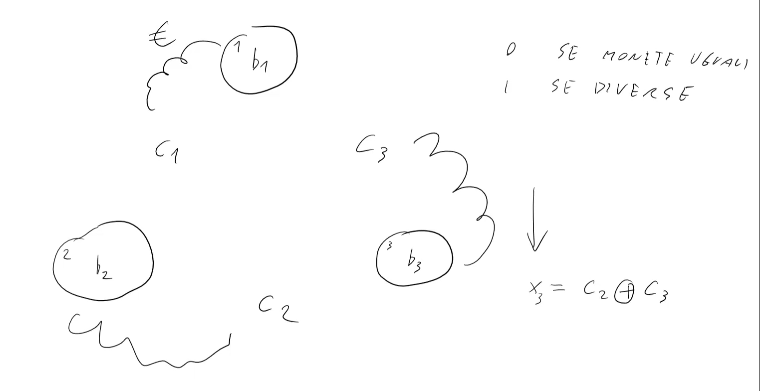
\includegraphics[width=1\textwidth]{images/12-3.png}
    \caption{Schema grafico del protocollo}
    \label{fig:12-3}
\end{figure}
\begin{enumerate}
    \item Abbiamo tre crittografi 1, 2, 3. Di conseguenza abbiamo $b_1, b_2, b_3$;
    \item Ogni crittografo lancia una moneta ($c_1, c_2, c_2$) alla propria destra. Ogni moneta è visibile solo dal crittografo che l'ha lanciata e da quello alla sua destra;
    \item Ogni crittografo vede due monete: quella che ha lanciato e quella alla sua sinistra;
    \item Ogni crittografo calcola $x$ dato dallo XOR delle monete che vede (es: $x_3 = c_2 \oplus c_3$);
    \item Ogni crittografo ottiene $0$ se le monete sono uguali o $1$ se sono diverse;
    \item Il crittografo che ha pagato complementa il proprio $x$;
    \item Ogni crittografo comunica il proprio risultato: solo il crittografo che ha pagato comunicherà l'opposto del risultato che ha ottenuto;
    \item Contando gli $0$ e gli $1$ i crittografi sono in grado di dire se uno di loro ha pagato o no.
\end{enumerate}

\noindent Come fanno i crittografi a dire se uno di loro ha pagato contando gli $0$ e gli $1$? Sappiamo che in condizioni normali (nessuno ha pagato) vale che
\begin{align*}
    x_1 \oplus x_2 \oplus x_3 = 0
\end{align*}

\noindent Se qualcuno paga allora il calcolo diventa:
\begin{align*}
    x_1 \oplus \bar{x_2} \oplus x_3 \equiv x_1 \oplus x_2 \oplus x_3 \oplus 1
\end{align*}

\noindent In quanto il complemento di un bit equivale a quel bit XOR $1$. Di conseguenza lo XOR dei tre bit annunciati dai crittografi ritorna $1$ al posto di $0$. 

Possiamo vederla in un altro modo. Contiamo quanto sono i bit a $1$ annunciati dai crittografi. Questi possono essere 0 o 2: sono 0 quando tutti i bit hanno lo stesso valore ($c_1 = c_2 = c_3$), sono 2 quando due valori sono uguali e uno è diverso (se $c_1 = c_3$, $b_1$ dirà $0$, $b_2$ e $b_3$ diranno $1$). Se un crittografo complementa il proprio bit, allora questi diventano o 1 o 3 (equivale a dire "lo XOR dà $1$"). 

Con questa funzioni tutti i crittografi sono in grado di calcolare la funzione. Se i crittografi che mentono sono due, allora questa funzione non va bene. Lavora bene solo se a pagare è solo un crittografo.
\\

\noindent Supponiamo che il risultato che otteniamo è $0$. Allora ogni crittografo sa che nessuno dei tre ha pagato. Ogni crittografo sa tutto degli altri crittografi. Non lo sa perché il protocollo gli ha rivelato informazioni aggiuntive, ma sa esattamente quello che può sapere conoscendo il proprio bit e il risultato della funzione. In questo caso, essendo il risultato $0$, conosce di conseguenza il valore del bit degli altri crittografi. 

Se il risultato della funzione è $1$, il crittografo che ha pagato sa tutto anche degli altri crittografi, mentre gli altri sanno solo che qualcuno tra loro ha pagato, ma non chi.
\\

\noindent Il protocollo è generalizzabile a $n$ crittografi (\ref{fig:12-3-1}). Come sopra $x_1 \oplus ... \oplus x_n = 0$, poiché ogni moneta viene conteggiata due volte. Tuttavia se un crittografo complementa il proprio bit, che equivale ad aggiungere un $\oplus 1$, il risultato diventa $1$. Questo sistema funziona solo se il numero di bit a $1$ è dispari (se è pari il loro XOR dà $0$).

\begin{figure}
    \centering
    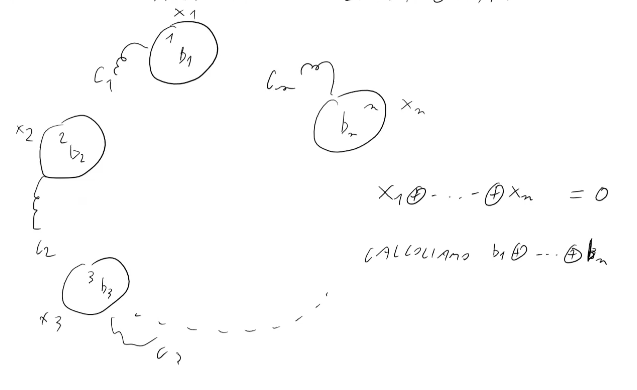
\includegraphics[width=1\textwidth]{images/12-3-1.png}
    \caption{Schema grafico del protocollo}
    \label{fig:12-3-1}
\end{figure}

\noindent A cosa ci può servire un protocollo del genere? Incarichiamo un solo crittografo di spedire un bit agli altri agenti. Il crittografo si comporta come il crittografo che ha pagato nel caso in cui il bit da spedire sia $1$. Gli altri crittografi osservano il bit trasmesso, ma non sanno il suo valore. 

Abbiamo creato una situazione in cui un crittografo può inviare un bit senza rivelare la propria identità.\\

\paragraph{Controllo del canale di comunicazione} Cambiamo contesto. Ora non c'è più un agente esterno che dice al crittografo di inviare il bit, ma è il crittografo che vuole inviare il bit in broadcast a tutti. Come fa a trasmettere? Supponiamo di avere un qualcosa che scaglioni il tempo. Quando scatta il tic i crittografi lanciano al moneta e la comunicano a lato. Al tic successivo i crittografi comunicano il valore di $x$. Un crittografo che vuole spedire un bit a $0$ non fa nulla (si comporta come un crittografo che non ha mangiato), mentre uno che vuole spedire $1$ si comporta come un crittografo che ha mangiato. Ad ogni coppia di tic, il crittografo che vuole trasmettere codifica il bit che vuole spedire. 

Supponiamo che il crittografo che trasmette sia uno solo. In questo caso riesce a trasmettere con successo e tutti vedono il risultato della trasmissione. Il crittografo può anche inviare una sequenza di bit. 

Potrebbero essere però presenti dei conflitti, ad esempio quando due crittografi decidono di spedire contemporaneamente. I due agenti hanno modo di accorgersi del conflitto? Ogni crittografo, quando spedisce il bit, riesce anche ad osservare il bit che è stato trasmesso sulla rete (lui, come tutti gli altri, fa lo XOR degli $x_i$). Se trasmette un bit e vede che nella rete c'è esattamente il bit che ha trasmesso, potrebbero anche esserci dei conflitti (se tre crittografi inviano $1$, il risultato è comunque $1$), ma non è un problema perché sta circolando il messaggio che volevamo.

Nel momento in cui c'è in circolo un altro bit diverso da nostro, uno dei due osserverà che il bit che sta circolando è diverso da quello che aveva inviato. Tutti i crittografi che si accorgono di aver creato un conflitto si fermano e lasciano continuare gli altri (simile al protocollo ethernet). 

Quindi se un crittografo vuole trasmettere, procede come segue:
\begin{itemize}
    \item Verifica che nessuno stia trasmettendo;
    \item Se il canale è vuoto inizia a trasmettere, continuando a controllare eventuali conflitti.
\end{itemize}

\paragraph{Invio del messaggio} Supponiamo ora che un crittografo $i$ voglia inviare un messaggio a un crittografo $j$. Poiché può trasmettere solo in broadcast, il messaggio conterrà l'identità del destinatario. Come possiamo nascondere il destinatario di un messaggio? Potremmo semplicemente prender il messaggio e cifrarlo con la chiave pubblica del destinatario. 
\\

\noindent Abbiamo realizzato un sistema di comunicazione completamente non tracciabile: non si sa chi ha inviato il messaggio, non si sa chi ha ricevuto il messaggio e non si sa qual è il contenuto del messaggio.

Si tratta comunque di un protocollo dispendioso, in quanto gli agente dovrebbe restare attivi durante tutte le fasi. Presenta inoltre un difetto: se un agente vuole oscurare il canale, lo può fare facilmente inviando bit casuali, senza che nessun altro agente sappia  che è lui (è debole al denial of service -> tinen il canale occupato e causa conflitti nel caso un altro agente invii un messaggio).